\section{Uncorrected Distributions}
\label{section: uncorrected_distributions}

The uncorrected distributions for track multiplicity of MC data, track multiplicity of measured data and track kinematic quantities (pseudorapidity ($\eta$), azimuthal angle ($\phi$) and transverse momentum ($p_T$) for MC and measured data are shown in figures \ref{fig: reconstructed track multiplicity mc down},  \ref{fig: reconstructed track multiplicity measured down} and \ref{fig: reconstructed track eta, phi, pt and p mag down} respectively. These plots are for data in the magnet down configuration only.

\begin{figure}[h]
	\begin{subfigure}[h]{0.32\textwidth}
		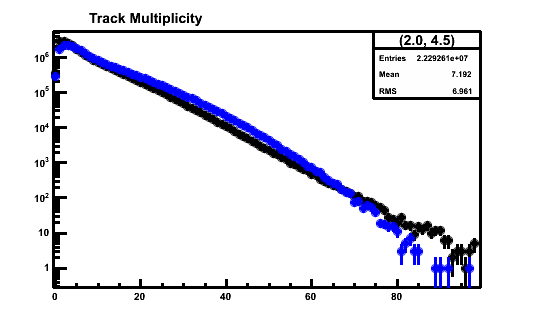
\includegraphics[width=\textwidth]{./Chapters/multiplicity/images/reconstructed_multiplicity_2_0_4_5_mc_down.png}
		\caption{$2.0 \le \eta < 4.5$}
		\label{fig: reconstructed track multiplicity mc down 2.0 - 4.5}
	\end{subfigure}
	\begin{subfigure}[h]{0.32\textwidth}
		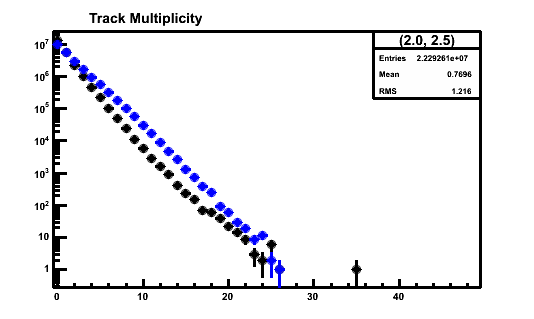
\includegraphics[width=\textwidth]{./Chapters/multiplicity/images/reconstructed_multiplicity_2_0_2_5_mc_down.png}
		\caption{$2.0 \le \eta < 2.5$}
		\label{fig: reconstructed track multiplicity mc down 2.0 - 2.5}
	\end{subfigure}
	\begin{subfigure}[h]{0.32\textwidth}
		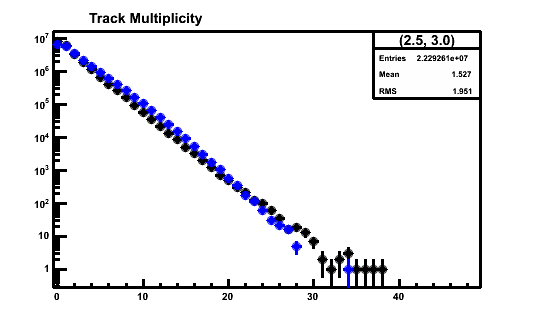
\includegraphics[width=\textwidth]{./Chapters/multiplicity/images/reconstructed_multiplicity_2_5_3_0_mc_down.png}
		\caption{$2.5 \le \eta < 3.0$}
		\label{fig: reconstructed track multiplicity mc down 2.5 - 3.0}
	\end{subfigure}
	\begin{subfigure}[h]{0.32\textwidth}
		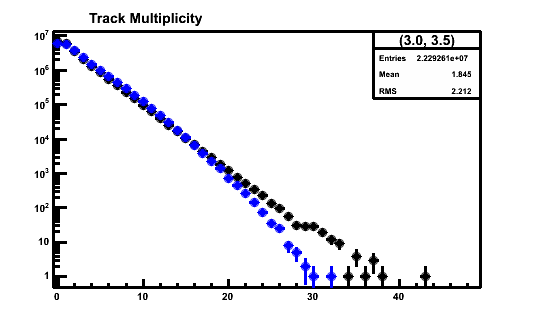
\includegraphics[width=\textwidth]{./Chapters/multiplicity/images/reconstructed_multiplicity_3_0_3_5_mc_down.png}
		\caption{$3.0 \le \eta < 3.5$}
		\label{fig: reconstructed track multiplicity mc down 3.0 - 3.5}
	\end{subfigure}
	\begin{subfigure}[h]{0.32\textwidth}
		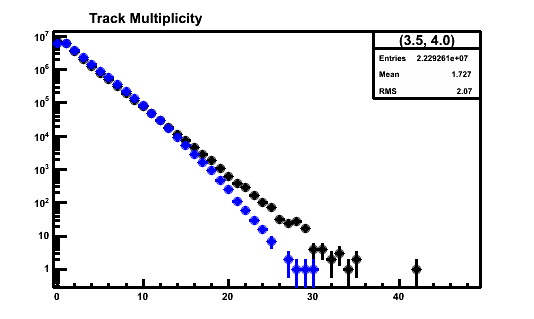
\includegraphics[width=\textwidth]{./Chapters/multiplicity/images/reconstructed_multiplicity_3_5_4_0_mc_down.png}
		\caption{$3.5 \le \eta < 4.0$}
		\label{fig: reconstructed track multiplicity mc down 3.5 - 4.0}
	\end{subfigure}
	\begin{subfigure}[h]{0.32\textwidth}
		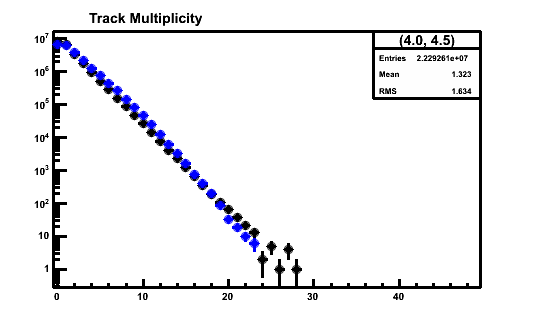
\includegraphics[width=\textwidth]{./Chapters/multiplicity/images/reconstructed_multiplicity_4_0_4_5_mc_down.png}
		\caption{$4.0 \le \eta < 4.5$}
		\label{fig: reconstructed track multiplicity mc down 4.0 - 4.5}
	\end{subfigure}
	\caption{Reconstructed track multiplicity of MC simulated data with the magnet down configuration sorted by $\eta$ region. The blue points correspond to the true particle multiplicity}
	\label{fig: reconstructed track multiplicity mc down}
\end{figure}

\begin{figure}[h]
	\begin{subfigure}[h]{0.32\textwidth}
		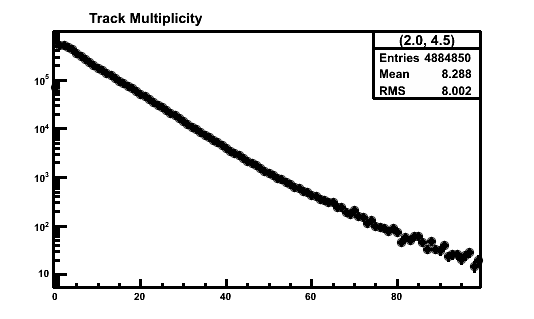
\includegraphics[width=\textwidth]{./Chapters/multiplicity/images/reconstructed_multiplicity_2_0_4_5_real_down.png}
		\caption{$2.0 \le \eta < 4.5$}
		\label{fig: reconstructed track multiplicity measured down 2.0 - 4.5}
	\end{subfigure}
	\begin{subfigure}[h]{0.32\textwidth}
		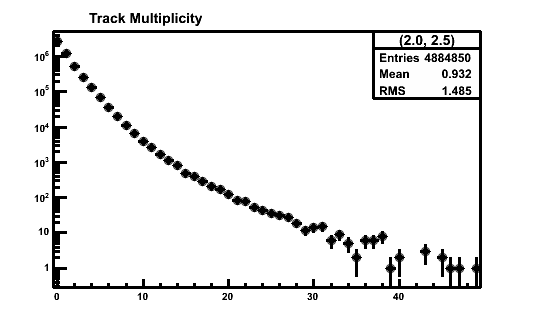
\includegraphics[width=\textwidth]{./Chapters/multiplicity/images/reconstructed_multiplicity_2_0_2_5_real_down.png}
		\caption{$2.0 \le \eta < 2.5$}
		\label{fig: reconstructed track multiplicity measured down 2.0 - 2.5}
	\end{subfigure}
	\begin{subfigure}[h]{0.32\textwidth}
		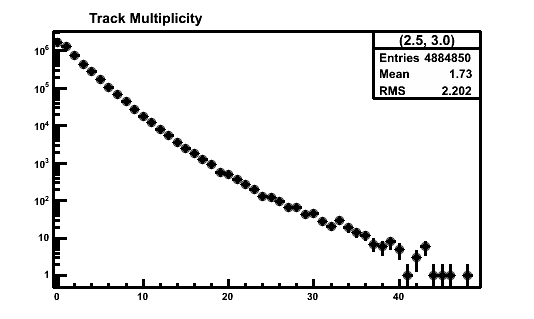
\includegraphics[width=\textwidth]{./Chapters/multiplicity/images/reconstructed_multiplicity_2_5_3_0_real_down.png}
		\caption{$2.5 \le \eta < 3.0$}
		\label{fig: reconstructed track multiplicity measured down 2.5 - 3.0}
	\end{subfigure}
	\begin{subfigure}[h]{0.32\textwidth}
		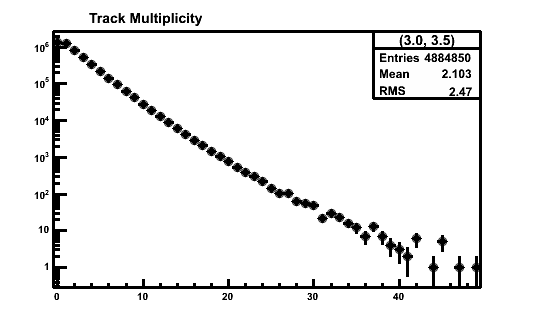
\includegraphics[width=\textwidth]{./Chapters/multiplicity/images/reconstructed_multiplicity_3_0_3_5_real_down.png}
		\caption{$3.0 \le \eta < 3.5$}
		\label{fig: reconstructed track multiplicity measured down 3.0 - 3.5}
	\end{subfigure}
	\begin{subfigure}[h]{0.32\textwidth}
		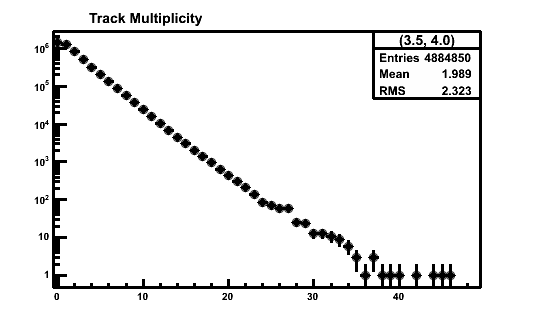
\includegraphics[width=\textwidth]{./Chapters/multiplicity/images/reconstructed_multiplicity_3_5_4_0_real_down.png}
		\caption{$3.5 \le \eta < 4.0$}
		\label{fig: reconstructed track multiplicity measured down 3.5 - 4.0}
	\end{subfigure}
	\begin{subfigure}[h]{0.32\textwidth}
		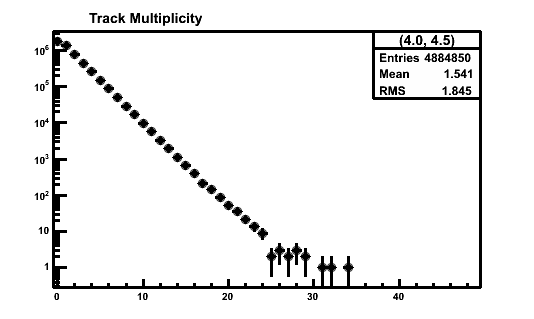
\includegraphics[width=\textwidth]{./Chapters/multiplicity/images/reconstructed_multiplicity_4_0_4_5_real_down.png}
		\caption{$4.0 \le \eta < 4.5$}
		\label{fig: reconstructed track multiplicity measured down 4.0 - 4.5}
	\end{subfigure}
	\caption{Reconstructed track multiplicity of measured data with the magnet down configuration sorted by $\eta$ region}
	\label{fig: reconstructed track multiplicity measured down}
\end{figure}

\begin{figure}[h]
	\begin{subfigure}[h]{0.49\textwidth}
		\includegraphics[width=\textwidth]{/afs/cern.ch/user/d/dvoong/cmtuser/DaVinci_v33r6/Phys/ChargedParticleMultiplicity/python/kinematic_distributions/tracks/data_files/plots/bk/Down/mc/-1/-1/bk/Down/mc/-1/-1/meissner/bk/Down/real/-1/-1/bk/Down/real/-1/-1/pngs/comparison/eta_comparison_norm.png}
		\caption{$\eta$}
		\label{fig: reconstructed eta mag down}
	\end{subfigure}
%	\begin{subfigure}[h]{0.49\textwidth}
%		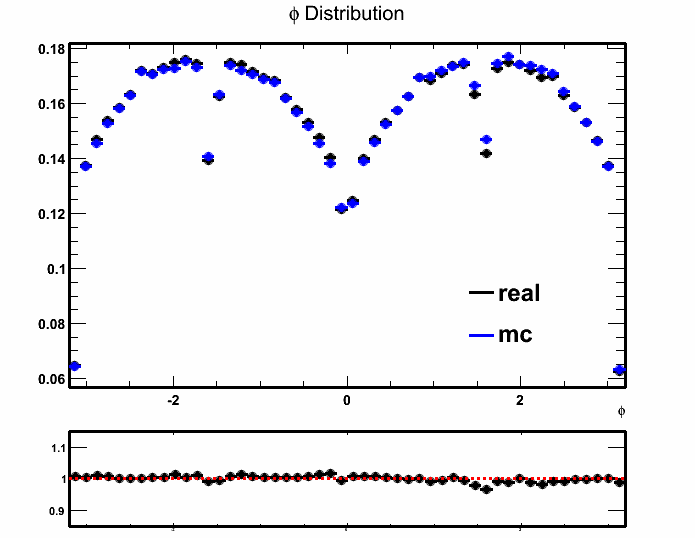
\includegraphics[width=\textwidth]{./Chapters/multiplicity/images/reconstructed_phi_mag_down.png}
%		\caption{$\phi$}
%		\label{fig: reconstructed phi mag down}
%	\end{subfigure}
	\centering
	\begin{subfigure}[h]{0.49\textwidth}
		\includegraphics[width=\textwidth]{/afs/cern.ch/user/d/dvoong/cmtuser/DaVinci_v33r6/Phys/ChargedParticleMultiplicity/python/kinematic_distributions/tracks/data_files/plots/bk/Down/mc/-1/-1/bk/Down/mc/-1/-1/meissner/bk/Down/real/-1/-1/bk/Down/real/-1/-1/pngs/comparison/pt_comparison_norm.png}
		\caption{$p_T$ (MeV)}
		\label{fig: reconstructed pt mag down}
	\end{subfigure}
%	\begin{subfigure}[h]{0.49\textwidth}
%		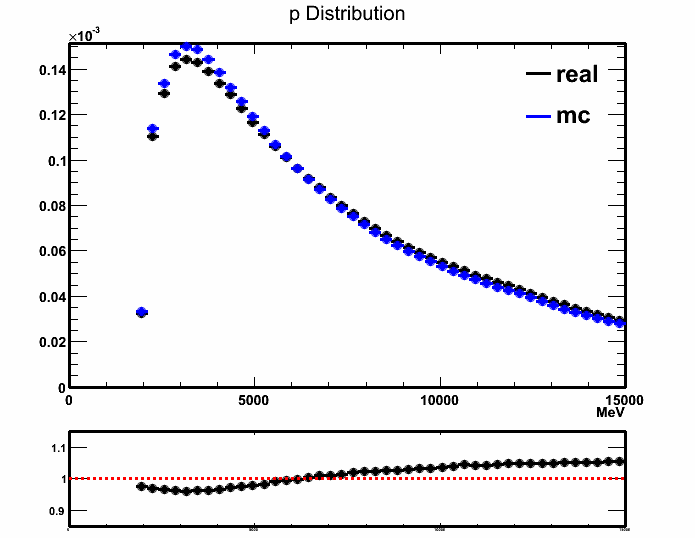
\includegraphics[width=\textwidth]{./Chapters/multiplicity/images/reconstructed_p_mag_down.png}
%		\caption{$|p|$ (MeV)}
%		\label{fig: reconstructed |p| mag down}
%	\end{subfigure}
	\caption{Uncorrected reconstructed track $\eta$ and $p_T$ of magnet down data. MC data is shown in blue.}
	\label{fig: reconstructed track eta, phi, pt and p mag down}
\end{figure}
